\PassOptionsToPackage{unicode=true}{hyperref} % options for packages loaded elsewhere
\PassOptionsToPackage{hyphens}{url}
\PassOptionsToPackage{dvipsnames,svgnames*,x11names*}{xcolor}
%
\documentclass[ignorenonframetext,]{beamer}
\usepackage{pgfpages}
\setbeamertemplate{caption}[numbered]
\setbeamertemplate{caption label separator}{: }
\setbeamercolor{caption name}{fg=normal text.fg}
\beamertemplatenavigationsymbolsempty
% Prevent slide breaks in the middle of a paragraph:
\widowpenalties 1 10000
\raggedbottom
\setbeamertemplate{part page}{
\centering
\begin{beamercolorbox}[sep=16pt,center]{part title}
  \usebeamerfont{part title}\insertpart\par
\end{beamercolorbox}
}
\setbeamertemplate{section page}{
\centering
\begin{beamercolorbox}[sep=12pt,center]{part title}
  \usebeamerfont{section title}\insertsection\par
\end{beamercolorbox}
}
\setbeamertemplate{subsection page}{
\centering
\begin{beamercolorbox}[sep=8pt,center]{part title}
  \usebeamerfont{subsection title}\insertsubsection\par
\end{beamercolorbox}
}
\AtBeginPart{
  \frame{\partpage}
}
\AtBeginSection{
  \ifbibliography
  \else
    \frame{\sectionpage}
  \fi
}
\AtBeginSubsection{
  \frame{\subsectionpage}
}
\usepackage{lmodern}
\usepackage{amssymb,amsmath}
\usepackage{ifxetex,ifluatex}
\usepackage{fixltx2e} % provides \textsubscript
\ifnum 0\ifxetex 1\fi\ifluatex 1\fi=0 % if pdftex
  \usepackage[T1]{fontenc}
  \usepackage[utf8]{inputenc}
  \usepackage{textcomp} % provides euro and other symbols
\else % if luatex or xelatex
  \usepackage{unicode-math}
  \defaultfontfeatures{Ligatures=TeX,Scale=MatchLowercase}
\fi
\usetheme[]{Singapore}
\usefonttheme{serif}
% use upquote if available, for straight quotes in verbatim environments
\IfFileExists{upquote.sty}{\usepackage{upquote}}{}
% use microtype if available
\IfFileExists{microtype.sty}{%
\usepackage[]{microtype}
\UseMicrotypeSet[protrusion]{basicmath} % disable protrusion for tt fonts
}{}
\IfFileExists{parskip.sty}{%
\usepackage{parskip}
}{% else
\setlength{\parindent}{0pt}
\setlength{\parskip}{6pt plus 2pt minus 1pt}
}
\usepackage{xcolor}
\usepackage{hyperref}
\hypersetup{
            pdftitle={Module 2, Part 2: Random vectors, covariance, multivariate Normal distribution},
            pdfauthor={Stefanie Muff, Department of Mathematical Sciences, NTNU},
            colorlinks=true,
            linkcolor=Maroon,
            filecolor=Maroon,
            citecolor=Blue,
            urlcolor=blue,
            breaklinks=true}
\urlstyle{same}  % don't use monospace font for urls
\newif\ifbibliography
\usepackage{color}
\usepackage{fancyvrb}
\newcommand{\VerbBar}{|}
\newcommand{\VERB}{\Verb[commandchars=\\\{\}]}
\DefineVerbatimEnvironment{Highlighting}{Verbatim}{commandchars=\\\{\}}
% Add ',fontsize=\small' for more characters per line
\usepackage{framed}
\definecolor{shadecolor}{RGB}{248,248,248}
\newenvironment{Shaded}{\begin{snugshade}}{\end{snugshade}}
\newcommand{\AlertTok}[1]{\textcolor[rgb]{0.94,0.16,0.16}{#1}}
\newcommand{\AnnotationTok}[1]{\textcolor[rgb]{0.56,0.35,0.01}{\textbf{\textit{#1}}}}
\newcommand{\AttributeTok}[1]{\textcolor[rgb]{0.77,0.63,0.00}{#1}}
\newcommand{\BaseNTok}[1]{\textcolor[rgb]{0.00,0.00,0.81}{#1}}
\newcommand{\BuiltInTok}[1]{#1}
\newcommand{\CharTok}[1]{\textcolor[rgb]{0.31,0.60,0.02}{#1}}
\newcommand{\CommentTok}[1]{\textcolor[rgb]{0.56,0.35,0.01}{\textit{#1}}}
\newcommand{\CommentVarTok}[1]{\textcolor[rgb]{0.56,0.35,0.01}{\textbf{\textit{#1}}}}
\newcommand{\ConstantTok}[1]{\textcolor[rgb]{0.00,0.00,0.00}{#1}}
\newcommand{\ControlFlowTok}[1]{\textcolor[rgb]{0.13,0.29,0.53}{\textbf{#1}}}
\newcommand{\DataTypeTok}[1]{\textcolor[rgb]{0.13,0.29,0.53}{#1}}
\newcommand{\DecValTok}[1]{\textcolor[rgb]{0.00,0.00,0.81}{#1}}
\newcommand{\DocumentationTok}[1]{\textcolor[rgb]{0.56,0.35,0.01}{\textbf{\textit{#1}}}}
\newcommand{\ErrorTok}[1]{\textcolor[rgb]{0.64,0.00,0.00}{\textbf{#1}}}
\newcommand{\ExtensionTok}[1]{#1}
\newcommand{\FloatTok}[1]{\textcolor[rgb]{0.00,0.00,0.81}{#1}}
\newcommand{\FunctionTok}[1]{\textcolor[rgb]{0.00,0.00,0.00}{#1}}
\newcommand{\ImportTok}[1]{#1}
\newcommand{\InformationTok}[1]{\textcolor[rgb]{0.56,0.35,0.01}{\textbf{\textit{#1}}}}
\newcommand{\KeywordTok}[1]{\textcolor[rgb]{0.13,0.29,0.53}{\textbf{#1}}}
\newcommand{\NormalTok}[1]{#1}
\newcommand{\OperatorTok}[1]{\textcolor[rgb]{0.81,0.36,0.00}{\textbf{#1}}}
\newcommand{\OtherTok}[1]{\textcolor[rgb]{0.56,0.35,0.01}{#1}}
\newcommand{\PreprocessorTok}[1]{\textcolor[rgb]{0.56,0.35,0.01}{\textit{#1}}}
\newcommand{\RegionMarkerTok}[1]{#1}
\newcommand{\SpecialCharTok}[1]{\textcolor[rgb]{0.00,0.00,0.00}{#1}}
\newcommand{\SpecialStringTok}[1]{\textcolor[rgb]{0.31,0.60,0.02}{#1}}
\newcommand{\StringTok}[1]{\textcolor[rgb]{0.31,0.60,0.02}{#1}}
\newcommand{\VariableTok}[1]{\textcolor[rgb]{0.00,0.00,0.00}{#1}}
\newcommand{\VerbatimStringTok}[1]{\textcolor[rgb]{0.31,0.60,0.02}{#1}}
\newcommand{\WarningTok}[1]{\textcolor[rgb]{0.56,0.35,0.01}{\textbf{\textit{#1}}}}
\usepackage{graphicx,grffile}
\makeatletter
\def\maxwidth{\ifdim\Gin@nat@width>\linewidth\linewidth\else\Gin@nat@width\fi}
\def\maxheight{\ifdim\Gin@nat@height>\textheight\textheight\else\Gin@nat@height\fi}
\makeatother
% Scale images if necessary, so that they will not overflow the page
% margins by default, and it is still possible to overwrite the defaults
% using explicit options in \includegraphics[width, height, ...]{}
\setkeys{Gin}{width=\maxwidth,height=\maxheight,keepaspectratio}
\setlength{\emergencystretch}{3em}  % prevent overfull lines
\providecommand{\tightlist}{%
  \setlength{\itemsep}{0pt}\setlength{\parskip}{0pt}}
\setcounter{secnumdepth}{0}

% set default figure placement to htbp
\makeatletter
\def\fps@figure{htbp}
\makeatother

\usepackage{xcolor}

\title{Module 2, Part 2: Random vectors, covariance, multivariate Normal
distribution}
\providecommand{\subtitle}[1]{}
\subtitle{TMA4268 Statistical Learning V2021}
\author{Stefanie Muff, Department of Mathematical Sciences, NTNU}
\date{January 19, 2021}

\begin{document}
\frame{\titlepage}

\begin{frame}

Last update: January 18, 2021

\end{frame}

\begin{frame}{Overview}
\protect\hypertarget{overview}{}

\normalsize

\begin{itemize}
\item
  Random vectors \vspace{2mm}
\item
  The covariance and correlation matrix \vspace{2mm}
\item
  The multivariate normal distribution
\end{itemize}

\end{frame}

\begin{frame}{Random vector}
\protect\hypertarget{random-vector}{}

\begin{itemize}
\tightlist
\item
  A random vector \(\boldsymbol{X}_{(p\times 1)}\) is a
  \(p\)-dimensional vector of random variables. For example

  \begin{itemize}
  \tightlist
  \item
    Weight of cork deposits in \(p=4\) directions (N, E, S, W).
  \item
    Factors to predict body fat: bmi, age, weight, hip
    circumference,\ldots{}.
  \end{itemize}
\item
  Joint distribution function: \(f(\boldsymbol{x})\).
\item
  From joint distribution function to marginal (and conditional
  distributions).
  \[f_1(x_1)=\int_{-\infty}^{\infty}\cdots \int_{-\infty}^{\infty} f(x_1,x_2,\ldots,x_p)dx_2 \cdots dx_p\]
\item
  Cumulative distribution (definite integrals!) used to calculate
  probabilites.
\item
  Independence: \(f(x_1,x_2)=f_1(x_1)\cdot f(x_2)\) and
  \(f(x_1\mid x_2)=f_1(x_1).\)
\end{itemize}

\end{frame}

\begin{frame}

\begin{block}{Moments}

\vspace{2mm}

The moments are important properties of the distribution of
\(\boldsymbol{X}\). We will look at:

\vspace{2mm}

\begin{itemize}
\tightlist
\item
  E: Mean of random vector and random matrices.
\item
  Cov: Covariance matrix.
\item
  Corr: Correlation matrix.
\item
  E and Cov of multiple linear combinations.
\end{itemize}

\end{block}

\end{frame}

\begin{frame}[fragile]

\begin{block}{The Cork deposit data}

\(~\)

\begin{itemize}
\tightlist
\item
  Classical multivariate data set from Rao (1948).
\item
  Weigth of bark deposits of \(n=28\) cork trees in \(p=4\) directions
  (N, E, S, W).
\end{itemize}

\(~\)

\tiny

\begin{Shaded}
\begin{Highlighting}[]
\NormalTok{corkds =}\StringTok{ }\KeywordTok{as.matrix}\NormalTok{(}\KeywordTok{read.table}\NormalTok{(}\StringTok{"https://www.math.ntnu.no/emner/TMA4268/2019v/data/corkMKB.txt"}\NormalTok{))}
\KeywordTok{dimnames}\NormalTok{(corkds)[[}\DecValTok{2}\NormalTok{]] =}\StringTok{ }\KeywordTok{c}\NormalTok{(}\StringTok{"N"}\NormalTok{, }\StringTok{"E"}\NormalTok{, }\StringTok{"S"}\NormalTok{, }\StringTok{"W"}\NormalTok{)}
\KeywordTok{head}\NormalTok{(corkds)}
\end{Highlighting}
\end{Shaded}

\begin{verbatim}
##       N  E  S  W
## [1,] 72 66 76 77
## [2,] 60 53 66 63
## [3,] 56 57 64 58
## [4,] 41 29 36 38
## [5,] 32 32 35 36
## [6,] 30 35 34 26
\end{verbatim}

\begin{Shaded}
\begin{Highlighting}[]
\KeywordTok{dim}\NormalTok{(corkds)}
\end{Highlighting}
\end{Shaded}

\begin{verbatim}
## [1] 28  4
\end{verbatim}

\end{block}

\end{frame}

\begin{frame}[fragile]

Look at the data (always the first thing to do):

\tiny

\begin{Shaded}
\begin{Highlighting}[]
\KeywordTok{library}\NormalTok{(GGally)}
\NormalTok{corkds <-}\StringTok{ }\KeywordTok{as.data.frame}\NormalTok{(corkds)}
\KeywordTok{ggpairs}\NormalTok{(corkds)}
\end{Highlighting}
\end{Shaded}

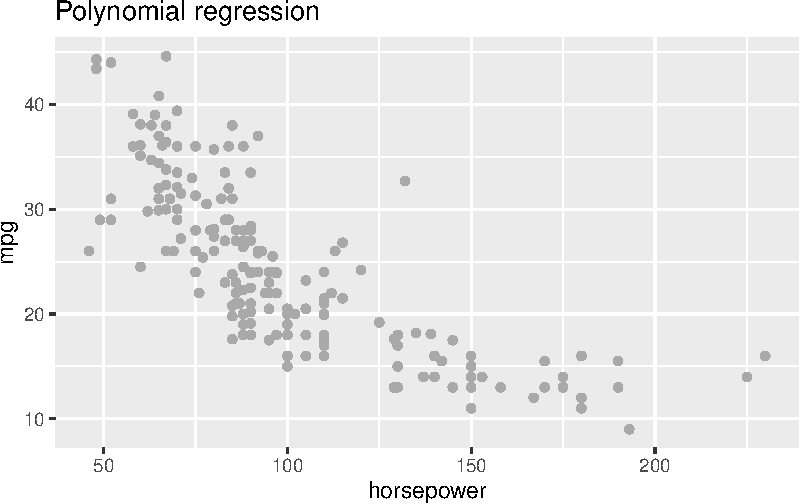
\includegraphics{2StatLearn.2_files/figure-beamer/unnamed-chunk-2-1.pdf}

\end{frame}

\begin{frame}

\begin{itemize}
\item
  Here we have a random sample of \(n=28\) cork trees from the
  population and observe a \(p=4\) dimensional random vector for each
  tree.
\item
  This leads us to the definition of random vectors and a random matrix
  for cork trees:
\end{itemize}

\[\boldsymbol{X}_{(28 \times 4)}=\left[ \begin{array}{cccc}X_{11} & X_{12} & X_{13}& X_{14}\\ X_{21} & X_{22} & X_{23}& X_{24}\\ X_{31} & X_{32} & X_{33}& X_{34}\\ \vdots & \vdots & \ddots & \vdots\\ X_{28,1} & X_{28,2} & X_{28,3}& X_{28,4}\\ \end{array} \right]\]

\end{frame}

\begin{frame}

\begin{block}{Rules for means}

\(~\)

\begin{itemize}
\tightlist
\item
  Random vector \(\boldsymbol{X}_{(p\times 1)}\) with mean vector
  \(\boldsymbol{\mu}_{(p\times 1)}\):\footnote{Observe that $\text{E}(X_j)$ is calculated from the marginal distribution of $X_j$ and contains no information about dependencies between $X_{j}$ and $X_k$, $k\neq j$.}
\end{itemize}

\[\boldsymbol{X}_{(p\times 1)}=\left[ \begin{array}{c}X_1\\ X_2\\ \vdots\\ X_p\\ \end{array}\right], \text{ and }\boldsymbol{\mu}_{(p \times 1)}=\text{E}(\boldsymbol{X})=\left[ \begin{array}{c}\text{E}(X_1)\\ \text{E}(X_2)\\ \vdots\\ \text{E}(X_p)\\ \end{array}\right] \ .\]

\begin{itemize}
\tightlist
\item
  Same rule for random matrices.
\end{itemize}

\vspace{2mm}

\begin{itemize}
\tightlist
\item
  Random matrix \(\boldsymbol{X}_{(n\times p)}\) and random matrix
  \(\boldsymbol{Y}_{(n\times p)}\):
  \[\text{E}(\boldsymbol{X}+\boldsymbol{Y})=\text{E}(\boldsymbol{X})+\text{E}(\boldsymbol{Y}) \ .\]
\end{itemize}

(Rules of vector addition)

\end{block}

\end{frame}

\begin{frame}

\begin{itemize}
\tightlist
\item
  Random matrix \(\boldsymbol{X}_{(n\times p)}\) and conformable
  constant matrices \(\boldsymbol{A}\) and \(\boldsymbol{B}\):
  \[\text{E}(\boldsymbol{A}\boldsymbol{X}\boldsymbol{B})=\boldsymbol{A}\text{E}(\boldsymbol{X})\boldsymbol{B}\]
\end{itemize}

Proof: Board

\vspace{60mm}

\end{frame}

\begin{frame}

\textbf{Q}:

\begin{itemize}
\tightlist
\item
  What are the univariate analogue to the formulas on the previous two
  slides (which you studied in your first introductory course in
  statistics)?
\end{itemize}

\vspace{80mm}

\end{frame}

\begin{frame}

\begin{block}{The covariance}

\vspace{2mm}

In the introductory statistics course we defined the covariance
\begin{align*}
\rho_{ij} & =\text{Cov}(X_i,X_j)  =\text{E}[(X_i-\mu_i)(X_j-\mu_j)] \\
& =\text{E}(X_i \cdot X_j)-\mu_i\mu_j \ . 
\end{align*}

\begin{itemize}
\tightlist
\item
  What is the covariance called when \(i=j\)?
\end{itemize}

\vspace{2mm}

\begin{itemize}
\tightlist
\item
  What does it mean when the covariance is

  \begin{itemize}
  \tightlist
  \item
    negative
  \item
    zero
  \item
    positive?
  \end{itemize}
\end{itemize}

\end{block}

\end{frame}

\begin{frame}

Make a scatter plot for negative, zero and positive correlation (see
also R example).

\vspace{6cm}

\end{frame}

\begin{frame}

\begin{block}{Variance-covariance matrix}

\vspace{2mm}

\begin{itemize}
\item
  Consider random vector \(\boldsymbol{X}_{(p\times 1)}\) with mean
  vector \(\boldsymbol{\mu}_{(p\times 1)}\):
  \[\boldsymbol{X}_{(p\times 1)} =\left[ \begin{array}{c} X_1\\ X_2\\ \vdots\\ X_p\\ \end{array} \right], \text{ and }\boldsymbol{\mu}_{(p\times 1)} =\text{E}(\boldsymbol{X})=\left[ \begin{array}{c} \text{E}(X_1)\\ \text{E}(X_2)\\ \vdots\\ \text{E}(X_p)\\ \end{array}\right]\]
\item
  Variance-covariance matrix \(\boldsymbol\Sigma\) (real and symmetric)
  \begin{align*}
  \boldsymbol\Sigma & =\text{Cov}(\boldsymbol{X})  
  =\text{E}[(\boldsymbol{X}-\boldsymbol{\mu})(\boldsymbol{X}-\boldsymbol{\mu})^T] \\
  & = \left[ \begin{array}{cccc} \sigma_{11} & \sigma_{12} & \cdots & \sigma_{1p}\\ \sigma_{12} & \sigma_{22} & \cdots & \sigma_{2p}\\ \vdots & \vdots & \ddots & \vdots\\ \sigma_{1p} & \sigma_{2p} & \cdots & \sigma_{pp}\\ \end{array}  \right] 
   = \text{E}(\boldsymbol{X}\boldsymbol{X}^T)-\boldsymbol{\mu}\boldsymbol{\mu}^T
  \end{align*}
\end{itemize}

\end{block}

\end{frame}

\begin{frame}

\begin{itemize}
\item
  The diagonal elements in \(\boldsymbol\Sigma\),
  \(\sigma_{ii}=\sigma_i^2\), are variances.
\item
  The off-diagonal elements are covariances
  \(\sigma_{ij}=\text{E}[(X_i-\mu_i)(X_j-\mu_j)]=\sigma_{ji}\).
\item
  \(\boldsymbol\Sigma\) is called variance, covariance and
  variance-covariance matrix and denoted both
  \(\text{Var}(\boldsymbol{X})\) and \(\text{Cov}(\boldsymbol{X})\).
\end{itemize}

\end{frame}

\begin{frame}

\begin{block}{Exercise: the variance-covariance matrix}

\vspace{2mm}

Let \(\boldsymbol{X}_{4\times 1}\) have variance-covariance matrix
\[\boldsymbol\Sigma= \left[ \begin{array}{cccc} 2&1&0&0\\
      1&2&0&1\\
      0&0&2&1\\
      0&1&1&2\\
          \end{array}
          \right].\]

Explain what this means.

\end{block}

\end{frame}

\begin{frame}

\begin{block}{Correlation matrix}

\(~\)

Correlation matrix \(\boldsymbol{\rho}\) (real and symmetric)
\[\boldsymbol{\rho}=\left[ \begin{array}{cccc}
    \frac{\sigma_{11}}{\sqrt{\sigma_{11}\sigma_{11}}} &
    \frac{\sigma_{12}}{\sqrt{\sigma_{11}\sigma_{22}}} &
    \cdots &
    \frac{\sigma_{1p}}{\sqrt{\sigma_{11}\sigma_{pp}}}\\
    \frac{\sigma_{12}}{\sqrt{\sigma_{11}\sigma_{22}}} &
    \frac{\sigma_{22}}{\sqrt{\sigma_{22}\sigma_{22}}} &
    \cdots &
    \frac{\sigma_{2p}}{\sqrt{\sigma_{22}\sigma_{pp}}}\\
    \vdots & \vdots & \ddots & \vdots\\
      \frac{\sigma_{1p}}{\sqrt{\sigma_{11}\sigma_{pp}}} &
    \frac{\sigma_{2p}}{\sqrt{\sigma_{22}\sigma_{pp}}} &
    \cdots &
    \frac{\sigma_{pp}}{\sqrt{\sigma_{pp}\sigma_{pp}}}\\ \end{array}\right]=
 \left[ \begin{array}{cccc}
    1 & \rho_{12} & \cdots & \rho_{1p}\\
    \rho_{12} & 1 & \cdots & \rho_{2p}\\
    \vdots & \vdots & \ddots & \vdots\\
    \rho_{1p} & \rho_{2p} & \cdots & 1\\
\end{array}\right]\]

\[\boldsymbol{\rho}=(\boldsymbol{V}^{\frac{1}{2}})^{-1}
    \boldsymbol\Sigma(\boldsymbol{V}^{\frac{1}{2}})^{-1}, \text{   where    }
   \boldsymbol{V}^{\frac{1}{2}}=
 \left[ \begin{array}{cccc}
    \sqrt{\sigma_{11}} & 0& \cdots & 0\\
    0 & \sqrt{\sigma_{22}} & \cdots & 0\\
    \vdots & \vdots & \ddots & \vdots\\
    0 & 0 & \cdots & \sqrt{\sigma_{pp}}\\
\end{array} \right]\]

\end{block}

\end{frame}

\begin{frame}

\begin{block}{Exercise: the correlation matrix}

\(~\)

Let \(\boldsymbol{X}_{4\times 1}\) have variance-covariance matrix
\[\boldsymbol\Sigma= \left[ \begin{array}{cccc} 2&1&0&0\\
      1&2&0&1\\
      0&0&2&1\\
      0&1&1&2\\
          \end{array}
          \right].\] Find the correlation matrix.

\end{block}

\end{frame}

\begin{frame}

\textbf{A}:

\end{frame}

\begin{frame}

\begin{block}{Linear combinations}

\(~\)

Consider a random vector \(\boldsymbol{X}_{(p\times 1)}\) with mean
vector \(\boldsymbol{\mu}=\text{E}(\boldsymbol{X})\) and
variance-covariance matrix
\(\boldsymbol\Sigma=\text{Cov}(\boldsymbol{X})\).

The linear combinations
\[\boldsymbol{Z}=\boldsymbol{C}\boldsymbol{X}=\left[ \begin{array}{c} \sum_{j=1}^p c_{1j}X_j\\ \sum_{j=1}^p c_{2j}X_j\\ \vdots \\ \sum_{j=1}^p c_{kj}X_j \end{array} \right]\]
have
\[\text{E}(\boldsymbol{Z})=\text{E}(\boldsymbol{C}\boldsymbol{X})=\boldsymbol{C}\boldsymbol{\mu}\]
\[\text{Cov}(\boldsymbol{Z})=\text{Cov}(\boldsymbol{C}\boldsymbol{X})=
   \boldsymbol{C}\boldsymbol\Sigma\boldsymbol{C}^T\]

\textbf{Exercise:} Follow the proof (board) - what are the most
important transitions?

\end{block}

\end{frame}

\begin{frame}

\begin{block}{Exercise: Linear combinations}

\[\boldsymbol{X}=\left[ \begin{array}{c} X_N\\
          X_E\\
X_S\\
          X_W\\
          \end{array}
          \right],
          \boldsymbol{\mu}=\left[
      \begin{array}{c} \mu_N\\
          \mu_E\\
\mu_S\\
          \mu_W\\
          \end{array}
          \right], \text{ and } \boldsymbol\Sigma=\left[ \begin{array}{cccc}
    \sigma_{NN} & \sigma_{NE} & \sigma_{NS} & \sigma_{NW}\\
    \sigma_{NE} & \sigma_{EE} & \sigma_{ES}& \sigma_{EW}\\
        \sigma_{NS} & \sigma_{EE} & \sigma_{SS}& \sigma_{SW}\\
    \sigma_{NW} & \sigma_{EW} & \sigma_{SW} & \sigma_{WW}\\
\end{array} \right]\]

Scientists would like to compare the following three \emph{contrasts}:
N-S, E+W and (E+W)-(N+S), and define a new random vector
\(\boldsymbol{Y}_{(3\times 1)}=\boldsymbol{C}_{(3\times 4)} \boldsymbol{X}_{(4\times 1)}\)
giving the three contrasts.

\vspace{2mm}

\begin{itemize}
\tightlist
\item
  Write down \(\boldsymbol{C}\).
\item
  Explain how to find \(\text{E}(Y_1)\) and \(\text{Cov}(Y_1,Y_3)\).
\item
  Use R to find the mean vector, covariance matrix and correlations
  matrix of \(\boldsymbol{Y}\), when the mean vector and covariance
  matrix for \(\boldsymbol{X}\) is given below.
\end{itemize}

\end{block}

\end{frame}

\begin{frame}[fragile]

\tiny

\begin{Shaded}
\begin{Highlighting}[]
\NormalTok{corkds <-}\StringTok{ }\KeywordTok{as.matrix}\NormalTok{(}\KeywordTok{read.table}\NormalTok{(}\StringTok{"https://www.math.ntnu.no/emner/TMA4268/2019v/data/corkMKB.txt"}\NormalTok{))}
\KeywordTok{dimnames}\NormalTok{(corkds)[[}\DecValTok{2}\NormalTok{]] <-}\StringTok{ }\KeywordTok{c}\NormalTok{(}\StringTok{"N"}\NormalTok{, }\StringTok{"E"}\NormalTok{, }\StringTok{"S"}\NormalTok{, }\StringTok{"W"}\NormalTok{)}
\NormalTok{mu =}\StringTok{ }\KeywordTok{apply}\NormalTok{(corkds, }\DecValTok{2}\NormalTok{, mean)}
\NormalTok{mu}
\NormalTok{Sigma =}\StringTok{ }\KeywordTok{var}\NormalTok{(corkds)}
\NormalTok{Sigma}
\end{Highlighting}
\end{Shaded}

\begin{verbatim}
##        N        E        S        W 
## 50.53571 46.17857 49.67857 45.17857 
##          N        E        S        W
## N 290.4061 223.7526 288.4378 226.2712
## E 223.7526 219.9299 229.0595 171.3743
## S 288.4378 229.0595 350.0040 259.5410
## W 226.2712 171.3743 259.5410 226.0040
\end{verbatim}

\begin{Shaded}
\begin{Highlighting}[]
\NormalTok{(C <-}\StringTok{ }\KeywordTok{matrix}\NormalTok{(}\KeywordTok{c}\NormalTok{(}\DecValTok{1}\NormalTok{, }\DecValTok{0}\NormalTok{, }\DecValTok{-1}\NormalTok{, }\DecValTok{0}\NormalTok{, }\DecValTok{0}\NormalTok{, }\DecValTok{1}\NormalTok{, }\DecValTok{0}\NormalTok{, }\DecValTok{1}\NormalTok{, }\DecValTok{-1}\NormalTok{, }\DecValTok{1}\NormalTok{, }\DecValTok{-1}\NormalTok{, }\DecValTok{1}\NormalTok{), }\DataTypeTok{byrow =}\NormalTok{ T, }\DataTypeTok{nrow =} \DecValTok{3}\NormalTok{))}
\end{Highlighting}
\end{Shaded}

\begin{verbatim}
##      [,1] [,2] [,3] [,4]
## [1,]    1    0   -1    0
## [2,]    0    1    0    1
## [3,]   -1    1   -1    1
\end{verbatim}

\begin{Shaded}
\begin{Highlighting}[]
\NormalTok{C }\OperatorTok\StringTok{ }\NormalTok{Sigma }\OperatorTok\StringTok{ }\KeywordTok{t}\NormalTok{(C)}
\end{Highlighting}
\end{Shaded}

\begin{verbatim}
##           [,1]       [,2]       [,3]
## [1,]  63.53439  -38.57672   21.02116
## [2,] -38.57672  788.68254 -149.94180
## [3,]  21.02116 -149.94180  128.71958
\end{verbatim}

\end{frame}

\begin{frame}

\begin{block}{The covariance matrix - more requirements?}

\(~\)

Random vector \(\boldsymbol{X}_{(p\times 1)}\) with mean vector
\(\boldsymbol{\mu}_{(p\times 1)}\) and covariance matrix
\[\boldsymbol\Sigma=\text{Cov}(\boldsymbol{X})=\text{E}[(\boldsymbol{X}-\boldsymbol{\mu})(\boldsymbol{X}-\boldsymbol{\mu})^T]=
\left[ \begin{array}{cccc}
    \sigma_{11} & \sigma_{12} & \cdots & \sigma_{1p}\\
    \sigma_{12} & \sigma_{22} & \cdots & \sigma_{2p}\\
    \vdots & \vdots & \ddots & \vdots\\
    \sigma_{1p} & \sigma_{2p} & \cdots & \sigma_{pp}\\
\end{array} \right]\]

\end{block}

\end{frame}

\begin{frame}

\begin{itemize}
\tightlist
\item
  The covariance matrix is by construction symmetric, and it is common
  to require that the covariance matrix is positive semidefinite. This
  means that, for every vector \(\boldsymbol{b}\neq \boldsymbol{0}\)
\end{itemize}

\[\boldsymbol{b}^T \boldsymbol{\Sigma} \boldsymbol{b} \geq 0 \ .\]

\begin{itemize}
\tightlist
\item
  Why do you think that is?
\end{itemize}

\(~\)

Hint: Is it possible that the variance of the linear combination
\(\boldsymbol{Y}=\boldsymbol{b}^T\boldsymbol{X}\) is negative?

\end{frame}

\begin{frame}

\begin{block}{Random vectors - Single-choice exercise}

\vspace{4mm}

We are doing a poll in zoom.

\end{block}

\end{frame}

\begin{frame}

\begin{block}{Question 1: Mean of sum}

\vspace{2mm}

\(\boldsymbol{X}\) and \(\boldsymbol{Y}\) are two bivariate random
vectors with \(\text{E}(\boldsymbol{X})=(1,2)^T\) and
\(\text{E}(\boldsymbol{Y})=(2,0)^T\). What is
\(\text{E}(\boldsymbol{X}+\boldsymbol{Y})\)?

\(~\)

\begin{itemize}
\tightlist
\item
  A: \((1.5,1)^T\)
\item
  B: \((3,2)^T\)
\item
  C: \((-1,2)^ T\)
\item
  D: \((1,-2)^T\)
\end{itemize}

\end{block}

\end{frame}

\begin{frame}

\begin{block}{Question 2: Mean of linear combination}

\vspace{2mm}

\(\boldsymbol{X}\) is a 2-dimensional random vector with
\(\text{E}(\boldsymbol{X})=(2,5)^T\) , and
\(\boldsymbol{b}=(0.5, 0.5)^T\) is a constant vector. What is
\(\text{E}(\boldsymbol{b}^T\boldsymbol{X})\)?

\(~\)

\begin{itemize}
\tightlist
\item
  A: 3.5
\item
  B: 7
\item
  C: 2
\item
  D: 5
\end{itemize}

\end{block}

\end{frame}

\begin{frame}

\begin{block}{Question 3: Covariance}

\vspace{2mm}

\(\boldsymbol{X}\) is a \(p\)-dimensional random vector with mean
\(\boldsymbol{\mu}\). Which of the following defines the covariance
matrix?

\(~\)

\begin{itemize}
\tightlist
\item
  A:
  \(E[(\boldsymbol{X}-\boldsymbol{\mu})^T(\boldsymbol{X}-\boldsymbol{\mu})]\)
\item
  B:
  \(E[(\boldsymbol{X}-\boldsymbol{\mu})(\boldsymbol{X}-\boldsymbol{\mu})^T]\)
\item
  C:
  \(E[(\boldsymbol{X}-\boldsymbol{\mu})(\boldsymbol{X}-\boldsymbol{\mu})]\)\\
\item
  D:
  \(E[(\boldsymbol{X}-\boldsymbol{\mu})^T(\boldsymbol{X}-\boldsymbol{\mu})^T]\)
\end{itemize}

\end{block}

\end{frame}

\begin{frame}

\begin{block}{Question 4: Mean of linear combinations}

\vspace{2mm}

\(\boldsymbol{X}\) is a \(p\)-dimensional random vector with mean
\(\boldsymbol{\mu}\) and covariance matrix \(\boldsymbol\Sigma\).
\(\boldsymbol{C}\) is a constant matrix. What is then the mean of the
\(k\)-dimensional random vector
\(\boldsymbol{Y}=\boldsymbol{C}\boldsymbol{X}\)?

\(~\)

\begin{itemize}
\tightlist
\item
  A: \(\boldsymbol{C}\boldsymbol{\mu}\)
\item
  B: \(\boldsymbol{C}\boldsymbol\Sigma\)
\item
  C: \(\boldsymbol{C}\boldsymbol{\mu}\boldsymbol{C}^T\)
\item
  D: \(\boldsymbol{C}\boldsymbol\Sigma\boldsymbol{C}^T\)
\end{itemize}

\end{block}

\end{frame}

\begin{frame}

\begin{block}{Question 5: Covariance of linear combinations}

\vspace{2mm}

\(\boldsymbol{X}\) is a \(p\)-dimensional random vector with mean
\(\boldsymbol{\mu}\) and covariance matrix \(\boldsymbol\Sigma\).
\(\boldsymbol{C}\) is a constant matrix. What is then the covariance of
the \(k\)-dimensional random vector
\(\boldsymbol{Y}=\boldsymbol{C}\boldsymbol{X}\)?

\(~\)

\begin{itemize}
\tightlist
\item
  A: \(\boldsymbol{C}\boldsymbol{\mu}\)
\item
  B: \(\boldsymbol{C}\boldsymbol\Sigma\)
\item
  C: \(\boldsymbol{C}\boldsymbol{\mu}\boldsymbol{C}^T\)
\item
  D: \(\boldsymbol{C}\boldsymbol\Sigma\boldsymbol{C}^T\)
\end{itemize}

\end{block}

\end{frame}

\begin{frame}

\begin{block}{Question 6: Correlation}

\vspace{2mm}

\(\boldsymbol{X}\) is a \(2\)-dimensional random vector with covariance
matrix \[ \boldsymbol\Sigma= \left[\begin{array}{cc}
          4 & 0.8 \\
          0.8 & 1\\
      \end{array}
    \right]\] Then the correlation between the two elements of
\(\boldsymbol{X}\) are:

\(~\)

\begin{itemize}
\tightlist
\item
  A: 0.10
\item
  B: 0.25
\item
  C: 0.40
\item
  D: 0.80
\end{itemize}

\end{block}

\end{frame}

\begin{frame}

\end{frame}

\begin{frame}{The multivariate normal distribution}
\protect\hypertarget{the-multivariate-normal-distribution}{}

\vspace{2mm}

Why is the mvN so popular?

\begin{itemize}
\tightlist
\item
  Many natural phenomena may be modelled using this distribution (just
  as in the univariate case).
\item
  Multivariate version of the central limit theorem- the sample mean
  will be approximately multivariate normal for large samples.
\item
  Good interpretability of the covariance.
\item
  Mathematically tractable.
\item
  Building block in many models and methods.
\end{itemize}

\end{frame}

\begin{frame}

\centering

\includegraphics[width=0.8\textwidth,height=\textheight]{mvN.jpeg}

3D multivariate Normal distributions

\end{frame}

\begin{frame}

\begin{block}{The multivariate normal (mvN) pdf}

\vspace{2mm}

The random vector \(\boldsymbol{X}_{p\times 1}\) is multivariate normal
\(N_p\) with mean \(\boldsymbol{\mu}\) and (positive definite) covariate
matrix \(\boldsymbol\Sigma\). The pdf is:

\[f(\boldsymbol{x})=\frac{1}{(2\pi)^\frac{p}{2}|\boldsymbol\Sigma|^\frac{1}{2}} \exp\{-\frac{1}{2}(\boldsymbol{x}-\boldsymbol{\mu})^T\boldsymbol\Sigma^{-1}(\boldsymbol{x}-\boldsymbol{\mu})\}\]
\(~\)

\textbf{Questions}:

\begin{itemize}
\item
  How does this compare to the univariate version?
  \[f(x)=\frac{1}{\sqrt{2\pi}\sigma}\exp\{ \frac{1}{2\sigma^2}(x-\mu)^2\}\]
\item
  Why do we need the constant in front of the \(\exp\)?
\item
  What is the dimension of the part in \(\exp\)?
\item
  What happens if the determinant \(|\boldsymbol\Sigma| = 0\)
  (degenerate case)? 
\end{itemize}

\end{block}

\end{frame}

\begin{frame}

\begin{block}{Four useful properties of the mvN}

\vspace{2mm}

Let \(\boldsymbol{X}_{(p\times 1)}\) be a random vector from
\(N_p(\boldsymbol{\mu},\boldsymbol\Sigma)\).

\vspace{2mm}

\begin{enumerate}
\item
  The grapical contours of the mvN are ellipsoids (can be shown using
  spectral decomposition).
\item
  Linear combinations of components of \(\boldsymbol{X}\) are
  (multivariate) normal
\item
  All subsets of the components of \(\boldsymbol{X}\) are (multivariate)
  normal (special case of the above).
\item
  Zero covariance implies that the corresponding components are
  independently distributed (in contrast to general distributions).
\end{enumerate}

\(~\)

\small

If you need a refresh, you might find that video useful:
\url{https://www.youtube.com/watch?v=eho8xH3E6mE}

\end{block}

\end{frame}

\begin{frame}

All of these are proven in TMA4267 Linear Statistical Models.

The result 4 is rather useful! If you have a bivariate normal and
observed covariance 0, then your variables are independent.

\end{frame}

\begin{frame}

\begin{block}{Contours of multivariate normal distribution}

\vspace{2mm}

\begin{itemize}
\item
  Contours of constant density for the \(p\)-dimensional normal
  distribution are ellipsoids defined by \(\boldsymbol{x}\) such that
  \[ (\boldsymbol{x}-\boldsymbol{\mu})^T\boldsymbol\Sigma^{-1}(\boldsymbol{x}-\boldsymbol{\mu})=b \]
  where \(b>0\) is a constant.
\item
  These ellipsoids are centered at \(\boldsymbol{\mu}\) and have axes
  \(\pm \sqrt{b \lambda_i}\boldsymbol{e}_i\), where
  \(\boldsymbol\Sigma\boldsymbol{e}_i=\lambda_i \boldsymbol{e}_i\)
  (eigenvector for \(\lambda_i\)), for \(i=1,...,p\).
\item
  To see this the spectral decomposition of the covariance matrix is
  useful.
\item
  \((\boldsymbol{x}-\boldsymbol{\mu})^T\boldsymbol\Sigma^{-1}(\boldsymbol{x}-\boldsymbol{\mu})\)
  is distributed as \(\chi^2_p\).
\end{itemize}

\end{block}

\end{frame}

\begin{frame}

Note:

\emph{In M4: Classification the mvN is very important and we will often
draw contours of the mvN as ellipses- and this is the reason why we do
that. }

\end{frame}

\begin{frame}

\begin{block}{Identify the mvNs from their contours}

\vspace{4mm}

Let
\(\boldsymbol\Sigma=\left[\begin{array}{cc} \sigma_x^2 & \rho\sigma_{x}\sigma_{y}\\\rho\sigma_{x}\sigma_{y}&\sigma_y^2\\ \end{array} \right]\).

\vspace{4mm}

The following four figure contours have been generated:

\begin{itemize}
\tightlist
\item
  1: \(\sigma_x=1\), \(\sigma_y=2\), \(\rho=-0.3\)
\item
  2: \(\sigma_x=1\), \(\sigma_y=1\), \(\rho=0\)
\item
  3: \(\sigma_x=1\), \(\sigma_y=1\), \(\rho=0.5\)
\item
  4: \(\sigma_x=1\), \(\sigma_y=2\), \(\rho=0\)
\end{itemize}

\vspace{8mm}

\textbf{Match the distributions to the figures on the next slide.}

\end{block}

\end{frame}

\begin{frame}

\begin{center}\includegraphics[width=0.65\linewidth]{2StatLearn.2_files/figure-beamer/cont-1} \end{center}

Take a look at the contour plots - when are the contours circles, when
ellipses?

\end{frame}

\begin{frame}

\begin{block}{Multiple choice - multivariate normal}

\vspace{2mm}

A second zoom poll.

Choose the correct answer. Let's go!

\end{block}

\end{frame}

\begin{frame}

\begin{block}{Question 1: Multivariate normal pdf}

\vspace{2mm}

The probability density function is
\((\frac{1}{2\pi})^\frac{p}{2}\det(\boldsymbol\Sigma)^{-\frac{1}{2}}\exp\{-\frac{1}{2}Q\}\)
where \(Q\) is

\vspace{2mm}

\begin{itemize}
\tightlist
\item
  A:
  \((\boldsymbol{x}-\boldsymbol{\mu})^T\boldsymbol\Sigma^{-1}(\boldsymbol{x}-\boldsymbol{\mu})\)
\item
  B:
  \((\boldsymbol{x}-\boldsymbol{\mu})\boldsymbol\Sigma(\boldsymbol{x}-\boldsymbol{\mu})^T\)
\item
  C: \(\boldsymbol\Sigma-\boldsymbol{\mu}\)
\end{itemize}

\end{block}

\end{frame}

\begin{frame}

\begin{block}{Question 2: Trivariate normal pdf}

\vspace{2mm}

What graphical form has the solution to \(f(\boldsymbol{x})=\) constant?

\vspace{2mm}

\begin{itemize}
\tightlist
\item
  A: Circle
\item
  B: Parabola
\item
  C: Ellipsoid
\item
  D: Bell shape
\end{itemize}

\end{block}

\end{frame}

\begin{frame}

\begin{block}{Question 3: Multivariate normal distribution}

\vspace{2mm}

\(\boldsymbol{X}_p \sim N_p(\boldsymbol{\mu},\boldsymbol\Sigma)\), and
\(\boldsymbol{C}\) is a \(k \times p\) constant matrix.
\(\boldsymbol{Y}=\boldsymbol{C}\boldsymbol{X}\) is

\vspace{2mm}

\begin{itemize}
\tightlist
\item
  A: Chi-squared with \(k\) degrees of freedom
\item
  B: Multivariate normal with mean \(k\boldsymbol{\mu}\)
\item
  C: Chi-squared with \(p\) degrees of freedom
\item
  D: Multivariate normal with mean \(\boldsymbol{C}\boldsymbol{\mu}\)
\end{itemize}

\end{block}

\end{frame}

\begin{frame}

\begin{block}{Question 4: Independence}

\vspace{2mm}

Let \(\boldsymbol{X}\sim N_3(\boldsymbol{\mu},\boldsymbol\Sigma)\), with
\[\boldsymbol\Sigma= \left[     
\begin{array}{ccc} 1&1&0\\
      1&3&2\\
      0&2&5\\
          \end{array}
          \right].\] Which two variables are independent?

\vspace{2mm}

\begin{itemize}
\tightlist
\item
  A: \(X_1\) and \(X_2\)
\item
  B: \(X_1\) and \(X_3\)
\item
  C: \(X_2\) and \(X_3\)
\item
  D: None -- but two are uncorrelated.
\end{itemize}

\end{block}

\end{frame}

\begin{frame}

\begin{block}{Question 5: Constructing independent variables?}

\vspace{2mm}

Let \(\boldsymbol{X}\sim N_p(\boldsymbol{\mu},\boldsymbol\Sigma)\). How
can I construct a vector of independent standard normal variables from
\(\boldsymbol{X}\)?

\vspace{2mm}

\begin{itemize}
\tightlist
\item
  A: \(\boldsymbol\Sigma(\boldsymbol{X}-\boldsymbol{\mu})\)
\item
  B: \(\boldsymbol\Sigma^{-1}(\boldsymbol{X}+\boldsymbol{\mu})\)
\item
  C:
  \(\boldsymbol\Sigma^{-\frac{1}{2}}(\boldsymbol{X}-\boldsymbol{\mu})\)
\item
  D:
  \(\boldsymbol\Sigma^{\frac{1}{2}}(\boldsymbol{X}+\boldsymbol{\mu})\)
\end{itemize}

\end{block}

\end{frame}

\begin{frame}

\end{frame}

\begin{frame}{ Further reading/resources}
\protect\hypertarget{further-readingresources}{}

\begin{itemize}
\tightlist
\item
  \href{https://www.youtube.com/playlist?list=PL5-da3qGB5IDvuFPNoSqheihPOQNJpzyy}{Videoes
  on YouTube by the authors of ISL, Chapter 2}
\end{itemize}

\end{frame}

\begin{frame}{Acknowledgements}
\protect\hypertarget{acknowledgements}{}

Thanks to Mette Langaas, who developed the first slide set in 2018 and
2019, and to Julia Debik for contributing to this module.

\end{frame}

\end{document}
